\documentclass{article}
\usepackage{amsmath}
\usepackage{amsfonts}
\usepackage{amssymb}
\usepackage{courier}
\usepackage{graphicx}
\usepackage{subfig}
\usepackage{listings}
\usepackage[margin=1in]{geometry}

\title{AlphaGo: Breakthrough in Machine Learning?}
\begin{document}
\nocite{*}


\begin{titlepage}
    \begin{center}
        \vspace*{2.5cm}
        {\bf Demystifying Google's AlphaGo}
        
        \vspace*{0.5cm}
        Artificial Intelligence II
        
        \vspace*{2.5cm}
        
        \begin{figure}[h]
        \centering
        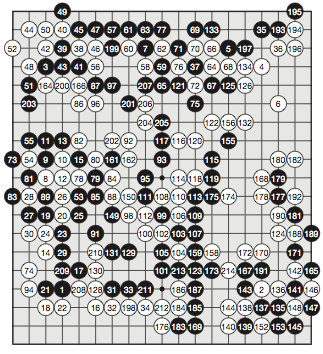
\includegraphics[width=11cm, height=11cm]{cover}
       \end{figure}
        
        \vspace{2.5cm}        
        
        \textbf{David Leonard}
	
	\vspace{0.5cm} 
	Date: May 2, 2016
        
        \vspace{1in}
        \vfill
        
    \end{center}
\end{titlepage}

\tableofcontents

\newpage

\section{Introduction}

Throughout the course of Artificial Intelligence I we have explored various game playing techniques which allow us to develop programs which can defeat human players for simple games such as Checkers. Through techniques such as Minimax evaluation, we were able to create an Artificial Intelligence which can compete with humans in Animal Shogi with the ability to look ahead $\approx 3$ turns. Using Minimax with Alpha-Beta Pruning, I was able to have 5-7 turn lookahead which allowed my program to compete on equal footing and even defeat most human players. 

Despite these improvements, tackling a game like Chess which has $35^{80}$ possible game states is not possible without more advanced heuristics and tree-pruning methods. While Chess has always been seen as a difficult game to master, it was done by IBM's Deep Blue which beat Chess world champion Garry Kasporav. At the time, this seemed to be a massive accomplishment for the field of Artificial Intelligence but as it turns out this accomplishment did not push forward any revolutionary changes. Recently, Google DeepMind has developed a program known as \textbf{AlphaGo} which was able to beat several high-dan ranking Go players across the world. Go has always been seen as a game whose state space was simply too massive to be explored ($250^{150}$ possible game states per turn). One possible solution to effectively prune sections of the game tree is to evaluate a given state $s$ and replace the subtree of $s$ with a value of an object function $v^*(s)$ which predicts the outcome of the game down state $s$ - similarly to how it was done with Alpha-Beta pruning. Unfortunately, this is believed to be impossible in Go due to the sheer size of the state space. 

Throughout the course of this paper, we will explore the methods used by AlphaGo to effectively handle Go as well as their Deep Learning architecture.

\section{Terminology}

In order to cope with the massive state space of Go, AlphaGo takes advantage of several methods for exploring and evaluating the current state of a game and training their architecture. We will define all of the terminology used in [1] here.

\subsection{Monte Carlo Tree Search}

Monte Carlo Tree Search is a heuristic akin to Alpha-Beta pruning in which the game tree is evaluated and helps to make decisions. The main idea of this heuristic is to expand the game state space using random sampling by playing out the entire game by selecting moves at random. Nodes in the game tree are updated with information regarding how many wins occurred after a fixed number of \textbf{playouts}, ultimately leading to the move which led to the most wins to in the simulation to be chosen. The steps for taken for this algorithm is stated below:

\begin{enumerate}
\item \textbf{Selection}: Start at the Root $R$ and select a random leaf node $L$. 
\item \textbf{Expansion}: If $L$ does not result in a win/loss, either create a new child node or choose a new node $C$.
\item \textbf{Simulation}: Run a fixed number of play outs.
\item \textbf{Backpropagate}: Update the nodes from path $C$ to $R$ with the play out results.
\end{enumerate}

Leaf nodes are selected carefully to strike a fair balance of \textbf{exploitation} of moves with high average win rates and \textbf{exploration} of moves with fewer simulations, akin to Simulated Annealing. The formula used for selecting $L$ is given by:

$$ \frac{w_{i}}{n_{i}} + c \sqrt{\frac{ln t}{n_i}}$$

Where $w_i$ is the number of wins after the $i-th$ move, $n_i$ is the number of simulations after the $i-th$ move, $c$ is the exploration parameter and $t$ is the number of simulations performed. At a first glance Monte Carlo Tree Search is similar to Minimax, however the benefit of this heuristic is that it is not tied to any evaluation function. Moreover, games with higher branching factors such as Chess and Go benefit from Monte Carlo Tree Search as the tree is built asymmetrically in order to explore more promising subtrees.

\begin{figure}[h]
\centering
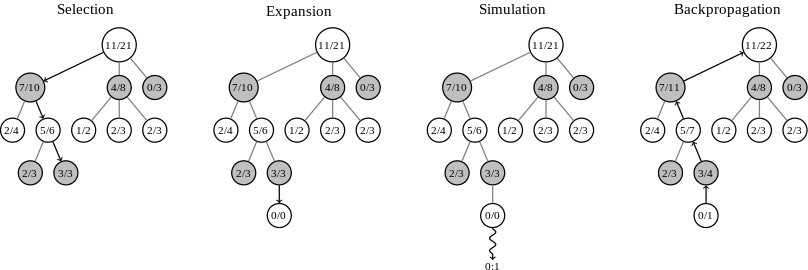
\includegraphics[width=16cm, height=8cm]{monte.png}
\caption{Monte Carlo Tree Search}
\end{figure}


\subsection{Convolutional Neural Networks}

Convolutional Neural Networks (CNN) are biologically-inspired variants of \textbf{Multi-Layer Perceptrons (MLP)} which are based off the visual cortex of animals. CNN's allow us to extract features (known as a \textbf{feature map}) from a 2D input (such as an image or speech signal). Not surprisingly, CNNs are based on \textbf{convolution} - where an input (more commonly an image) is convoluted with a linear filter. By repeatedly applying a function across sliding windows of an image, we can extract a feature map $h^k$:

$$h^{k}_{ij} = tanh((W^k * x)_{ij} + b_k)$$

Where each \textbf{hidden layer} is composed of multiple feature maps $ \{ h^{k}, = 0, 1, ..., K \}$ in order to get a better representation of the data. The weights $W$ of a CNN hidden layer is represented by a 4D tensor containing elements from every combination of the destination feature map, the source feature map, the source vertical position and source horizontal position, which can be visualized below. 

\begin{figure}[h]
\centering
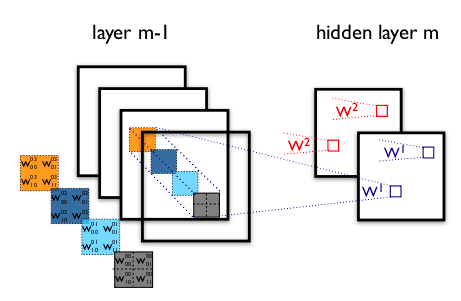
\includegraphics[width=6cm, height=4cm]{CCNW}
\caption{Representation of CNN}
\end{figure}

\newpage

At a high level, it is useful to understand that each layer in the CNN extracts more and more features. 

\begin{figure}[h]
\centering
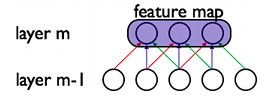
\includegraphics[width=8cm, height=3cm]{map}
\caption{Feature Map in CNN Layer}
\end{figure}

One example would be a three-layer CNN for recognizing faces, where the first layer will extract low level features, the second layer will extract mid-level features, and the last layer will extract high-level features. One such example is shown below in which a CNN is used to act as an edge detector of a true-color image:

\begin{figure}[h]
\centering
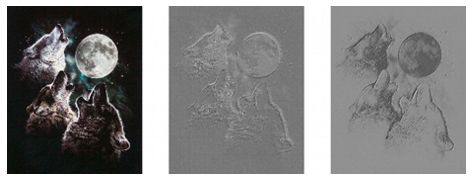
\includegraphics[width=16cm, height=6cm]{edge}
\caption{Feature Extraction from True Color Image}
\end{figure}

\subsection{Policy Network}

A \textbf{Policy Network} is simply a list or sample of moves to try at a given board position $s$, where the term $p(a|s)$ represents the probability distribution of all legal moves $a$ at board position $s$. This probability distribution is produced by a final \textbf{Softmax Layer}, which essentially maps a vector of size $K$ consisting of real values to a vector with real values between [0, 1] which adds up to 1. The end goal of the policy network is to be able to derive the best moves to try with a human vantage point.

\subsection{Value Network}

Value Networks are simply position evaluations, which again is trained using various CNN layers and outputs a scalar value $v_{\theta}(s')$ which represents the expected outcome in board position $s'$.

\section{Training Pipeline}

In this section, we will deep dive into the training pipeline which powers AlphaGo. We begin with looking into the \textbf{Supervised learning} of the \textbf{policy network}, followed by the \textbf{Reinforcement learning} of the \textbf{policy network} and lastly \textbf{Reinforcement learning} of the \textbf{Value network}.

\begin{figure}[h]
\centering
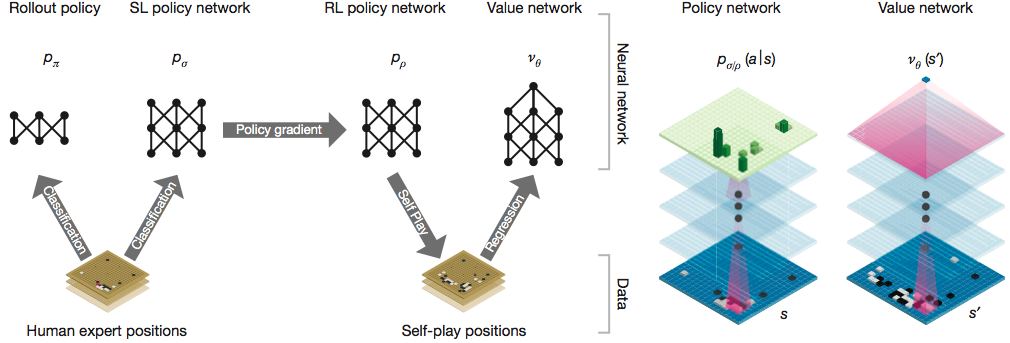
\includegraphics[width=16cm, height=6cm]{training}
\caption{Training Pipeline}
\end{figure}

\subsection{Supervised learning of the Policy Network}

The main driving force behind AlphaGo is it's ability to predict expert moves in Go, which has been an ongoing topic among various researchers. AlphaGo builds on top of past work to create a Supervised Learning Policy Network whose inputs $s$ is a simple representation of the board state with weight $\sigma$ The network is trained on randomly sampled state-action pairs $(s, a)$ using a method known as \textbf{stochastic gradient ascent}:

$$\Delta \sigma \propto \frac{\partial log P_\sigma (a|s)}{\partial \sigma}$$ 

The end result of this process is to maximize the chances of a human move $a$ being played at board state $s$. This is similar to being given a random board state in Chess, and trying to get checkmate in a fixed amount of turns (based on Chess puzzle books). By repeatedly training the policy network in such a way, it learns human moves based on a given situation. This network was trained using a 13-layer CNN using 30 million different positions.

\subsection{Reinforcement Learning of Policy Networks}

Once the policy network has been trained, it is now time for it to allow it to learn on it's own using \textbf{Reinforcement Learning} (also known as \textbf{Unsupervised Learning}). Reinforcement learning follows these steps:

\begin{enumerate}
\item {A set of environment states $S$, which is the set of board states $s$ in this case.}
\item {A set of actions $A$, which is the set of legal moves $a$ in this case.}
\item {A set of rules transitioning between states, i.e transitioning from board state $s$ to $s'$ using $a$.}
\item {Rules that determine a scalar reward of a transition, which is the output of the softmax layer}.
\item {Rules that describe what the agent (policy network) observes}.
\end{enumerate}

In order to train the Policy Network $p$ using Reinforcement Learning, it plays against a randomly chosen iteration of the policy network. The advantage of this method is that it prevents the policy network from overfitting to the current policy. A reward function $r(s)$ is used to present a scalar award based on whether the network won or list. The input weights $\sigma$ are updated once again using stochastic gradient ascent to maximize the expected outcome of human moves. Overall, the reinforcement learning policy network won more than 80\% of it's games against the supervised learning policy network. It was also able to beat the strongest open-source Go program, \textbf{Pachi} which executes 100,000 simulations per move. Without any search, the reinforcement learning policy network won 85\% of games against Pachi which is remarkable to say the least.

\subsection{Reinforcement Learning of Value Networks}

The final step of the training pipeline is to evaluate given positions on a board state $s$ by estimating the value function $v^p(s)$ which will predict the outcome from board state $s$ using the policy $p$. Since computing the optimal value function under perfect play is infeasible, it is instead estimated using the strongest policy $p_p$ from the Reinforcement Learning policy network. 

The architecture of this neural network is similar to the policy network, but it instead outputs a single prediction rather than a probability distribution $p$ and is instead trained using regression with state-outcome pairs $(s, z)$ using stochastic gradient descent. One major pitfall of training the value network this way is that it led to overfitting, causing the network to memorize outcomes and not generalize to new positions. To fix this, the network was retrained using a new dataset consisting of 30 million different positions which were all sampled from separate games. These games were then played between the reinforcement learning policy network and itself, leading to a decrease in error and overfitting. 

\subsection{Fast Rollout Policy}

In order to speed up the policy network, a faster but less accurate rollout policy $p_\pi(a|s)$ 
was also trained using linear softmax of smaller pattern features with weights $\pi$, whose accuracy was roughly 24.2\% in 2 $\mu s$ to select an action compared to 3ms for the original policy network. Recall that the rollout phase is when a game is simulated until the end from a selected node in the game tree.

\section{Searching using Policy and Value Networks}

Once the training is done, we now observe how searching through the game tree takes place. Monte Carlo Tree Search is used in combination with both the policy and value network which will select actions. Each edge of the tree is evaluated using both the value network $v_\theta$ and then by running the rollout using $p_\pi$ (the fast rollout policy) and finally computing the winner. The \textbf{Action value} \textbf{Q} stores the mean value of all the evaluations in the subtree below the given action. Each leaf in the game tree is evaluated using a random rollout which is played using $p_\pi$, and finally all the edges in the tree that were traversed are updated with these values. The algorithm culminates by selecting the most visited move from the root position.

\begin{figure}[h]
\centering
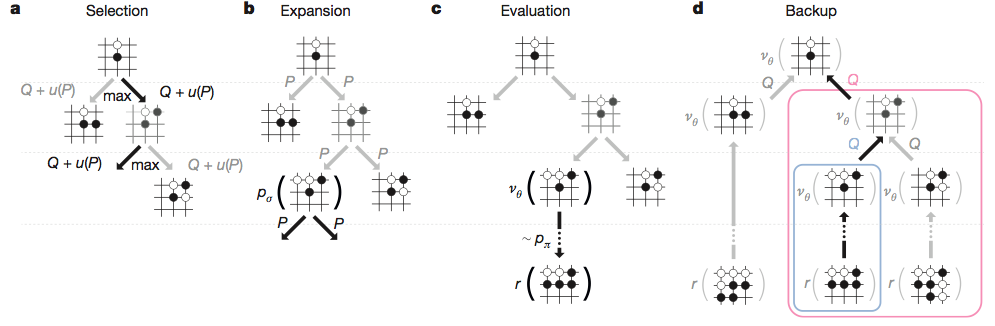
\includegraphics[width=16cm, height=6cm]{eval}
\caption{Searching with Policy and Value networks}
\end{figure}

\section{Hardware}

In order to utilize the power of this algorithm, AlphaGo uses asynchronous multi-threaded search which executes simulations on CPUs while the policy and value networks are trained in parallel on GPUs. In total, AlphaGo used 40 search threads, 48 CPUs and 8 GPUs. 

\section{Rankings}

In order to determine how strong AlphaGo was, it was pitted against the strongest Go programs to date which are all based off of Monto Carlo Tree Search Algorithms. Each program was given 5 seconds of computation time per move. 

\begin{figure}[h]
\centering
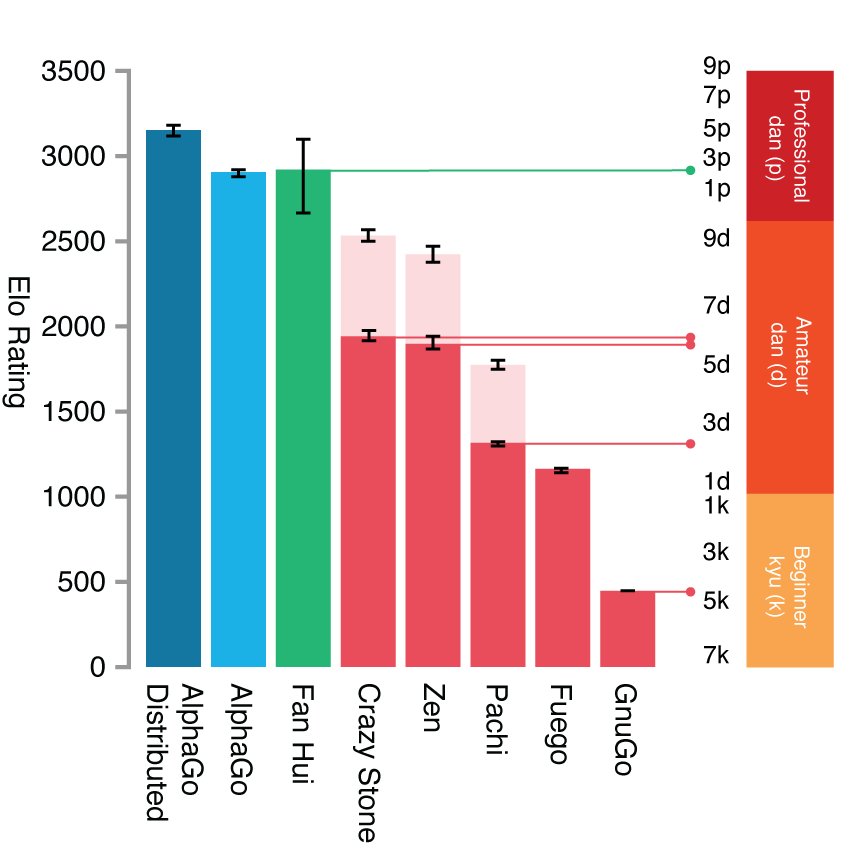
\includegraphics[width=12cm, height=10cm]{tourn}
\caption{Go Programs Tournament Results}
\end{figure}

The results show that AlphaGo is several \emph{dan} ranks stronger than all other programs (dan refers to how skilled a player is, where 9-dan is the best). Even when other programs were given handicaps to have free moves AlphaGo won with remarkable rates of 77\% (against Crazy Stone), 86\% (against Zen) and 99\% (against Pachi). The distributed version of AlphaGo (40 search threads, 1,202 CPUs and 176 GPUs) won 76\% of games against the lone AlphaGo and 100\% of games against all other programs. With AlphaGo's dominating performance over other \emph{programs}, it moved on to challenging world-ranking human players.

\section{AlphaGo versus Go Champions}

At the time of [1], AlphaGo played the European Go Champion Fan Hui and won 4 out of 5 games. This was an amazing feat, as mastering the game of Go has longly been considered a major challenge for Artificial Intelligence. An even greater feat is that during these matches, AlphaGo evaluated thousands of times fewer positions than Deep Blue did when playing Chess champion Garry Kasporov by selecting moves more intelligently through the use of it's policy network and evaluating them through the value network. Moreover, Deep Blue was trained using specific hardware and handcrafted evaluation functions, while the deep neural networks of AlphaGo were trained through gameplay using general-purpose supervised and reinforcement learning. Putting it all together, AlphaGo plays at a human level and is an amazing breakthrough in the field of Artificial Intelligence. By observing that AlphaGo triumphs over a game with tough decision making, an intractable search space and optimal solution, it gives hope that we may be able to attain human-level performance in other fields previously thought impossible.

Even more amazing is that recently (March 2016), AlphaGo went toe to toe with 18-time World Go Champion Lee Se-dol in a 5-game series, winning 4-1. In the game of Go, there are moves considered to be \emph{divine} such that the probability of finding these moves are 
incredibly small which were selected by AlphaGo. In fact, Lee Se-dol beat AlphaGo in Game 4 of the series using a divine move which was amazing in itself. Another testament to the power of AlphaGo is it was confident in it's ability to win at roughly the midpoint of each game, while the commentators themselves had no idea which player would come out on top.

\section{AlphaGo's Future}

Currently, AlphaGo's implementation is planned to be done on the \textbf{TensorFlow}\footnote{TensorFlow: https://www.tensorflow.org/} library - which is Google's open-source deep learning framework. Surprisingly, the release of Tensorflow seemed to make me believe that AlphaGo was built using it which is not the case. Researchers believe that implementing AlphaGo using TensorFlow will lead to more groundbreaking results. Google DeepMind is currently using the same architecture as AlphaGo to make breakthroughs in the healthcare domain \footnote{DeepMind tackles Healthcare: https://deepmind.com/health.html}.

\section{Conclusion}

Overall, AlphaGo is an amazing breakthrough in the field of Artificial Intelligence and I truly believe that it opens doors for human-level behavior in other domains (possibly human-esque robots that can cook?). Despite this, it may still be years (even decades) before we begin to see Artificial Intelligence at the levels we are accustomed to in cinema and fiction, but perhaps Google DeepMind's AlphaGo will start to revolutionize fields such as healthcare. 

\newpage

\begin{thebibliography}{9}
\bibitem{latexcompanion} 
David Silver et. al.
\textit{Mastering the game of Go with deep neural networks and tree search}. 
(doi:10.1038/nature16961) January 28, 2016.
 
 
\bibitem{einstein} 
Campbell, M., Hoane, A,  Hsu, F.
\textit{Deep Blue}.
Artif. Intell. 134, 57�83 (2002).
 
 
\bibitem{einstein} 
Google Research Blog
\textit{What we learned in Seoul with AlphaGo}.
https://goo.gl/bTT19m March 16, 2016.

\end{thebibliography}

\end{document}
